\newpage
\section{Architettura dei Processori moderni}
La classica architettura di un processore, riguardo l'esecuzione delle istruzioni, è poco efficiente, poichè bisogna aspettare sempre il termine di un istruzione per eseguire quella successiva.
Per velocizzare tale tipologia di sistema abbiamo 2 principali strade:
\begin{itemize}
    \item \textbf{Elettronicamente}: Si aumenta la frequenza di clock all'interno del nostro sistema (in gergo si utilizza il termine Overclock). Tale soluzione, per quanto semplice, è molto pericolosa, poichè dopo una certa soglia, non posso più aumentare la frequenza di clock. Aumentare troppo il clock potrebbe far danneggiare i componenti per la troppa energia da dissipare e quindi bisognerebbe prevedere anche delle architetture costruite ad-hoc;
    
    \item \textbf{Architetturalmente}: Vado a modificare l'architettura per gestire un nuovo modo di funzionamento del classico flusso di funzionamento di un processore. Tale modifica permetterebbe di poter eseguire più istruzioni contemporaneamente. Le tipologie di approcci che si possono avere in base a questa soluzione sono 2:
    \begin{itemize}
        \item \textbf{Parallelismo livello di Processo}: Ho a disposizione più processori (parallelismo esplicito) che vanno ad eseguire in maniera concorrente tali processi;
        \item \textbf{Parallalismo livello istruzione}: Un singolo processore riesce ad eseguire più istruzioni in maniera parallela;
    \end{itemize}
\end{itemize}

Le due macrosoluzioni non sono mutuamente esclusive, quindi si potrebbe anche pensare di effettuare una combinazione di esse.
Guardando nello specifico alla soluzione di tipo \textbf{Architetturale} si possono incontrare varie strade per poter implementare il parallelismo delle istruzioni.
Per poter meglio comprendere come effettuare la suddivisione del lavoro tramite le varie architetture, bisogna comprendere bene come strutturare un \textbf{Processo}. Tale entità la possiamo vedere come:
\begin{itemize}
    \item Formata da più task disgiunti ed indipendenti;
    \item Formata da un solo programma che richiede un'esecuzione ad elevate prestazioni.
\end{itemize}

Le architetture che negli anni sono state progettate per la distribuzione del carico di lavoro, dato da un singolo processo sono varie (quindi ci troviamo nel secondo caso).
Le tipologie principali sono:
\begin{itemize}
    \item \textbf{SISD (Single Istruction Single Data)}: Architettura in grado di eseguire una istruzione alla volta lavorando su dati singoli. Tale tipologia di architettura rispetta per filo e per segno la classica architettura di Von Neumann, la tipologia di parallelismo che si può implementare su tali sistemi è solo tramite un cambio di contesto, quindi definendo uno scheduling.
    \item \textbf{SIMD (Single Istruction Multiple Data)}: Architettura progettata per l'esecuzione di una singola istruzione su più dati. Tale tipologia di architettura è molto buona per l'esecuzione di prodotti vettoriali. Il parallelismo di tale macchina è intrinseco rispetto ai dati, poichè si agisce effettuando una singola istruzione sui vari dati.
    \item \textbf{MISD (Multiple Istruction Single Data)}: (Tali architetture sono state aggiunte solo per conoscenza personale, ma non sono state spiegate dal professore) Architettura in grado di eseguire una moltitudine di istruzioni su di un singolo dato. Tale tipologia di architettura è la meno utilizzata, poichè si cerca di eseguire sempre delle operazioni contemporanee rispetto ai dati.
    \item \textbf{MIMD (Multiple Istruction Multiple Data)}: Architettura che consente di eseguire più istruzioni su più dati. Essi eseguono quindi in parallelo, più istruzioni diverse su più dati diversi. Esse sono le più complicate per via della condivisione della memoria, difatti, ve ne sono varie, in base a come si vadano ad accedere i vari dati in memoria.
\end{itemize}

Nel nostro caso, il Motorola 68k è una tipologia di sistema \textbf{SISD}.
Ad oggi i sistemi maggiormente utilizzati sono i sistemi \textbf{MIMD}, che prevedono l'utilizzo di più unità di elaborazione per poter determinare uno specifico risultato. Tali sistemi, come detto in precedenza, possono essere di vario tipo e possono essere strutturati in vario modo.
Un primo approccio è quello di costruire due sistemi "gemelli", ovvero, costruire due calcolatori differenti che tramite la comunicazione I/O gestiscono le varie operazioni da effettuare. Tale sistema, però, non è molto efficente, poichè le comunicazioni tramite dispositivi di I/O non è veloce come i processori, per cui si avrebbe un rallentamento delle operazioni.
Per sopperire a tale problema, allora si potrebbe pensare di utilizzare un sistema di memoria condivisa tra i due processori, in modo da evitare i dispositivi di I/O. La problematica che si andrebbe a presentare in quest'altro caso sarebbe l'accesso al BUS, che nonostante sia velocissimo, ha bisogno di una buona comunicazione tra i due processori.
Per migliorare ancora tale tipologia di architettura, allora, si potrebbe pensare di utilizzare una gerarchia di memorie, che permetta di ridurre gli accessi in memoria pilotati dai vari processori, che possono lavorare sulle loro memoria "private" in maniera del tutto autonoma e concorrente senza dover schedulare l'accesso al BUS.

\begin{figure}
    \centering
    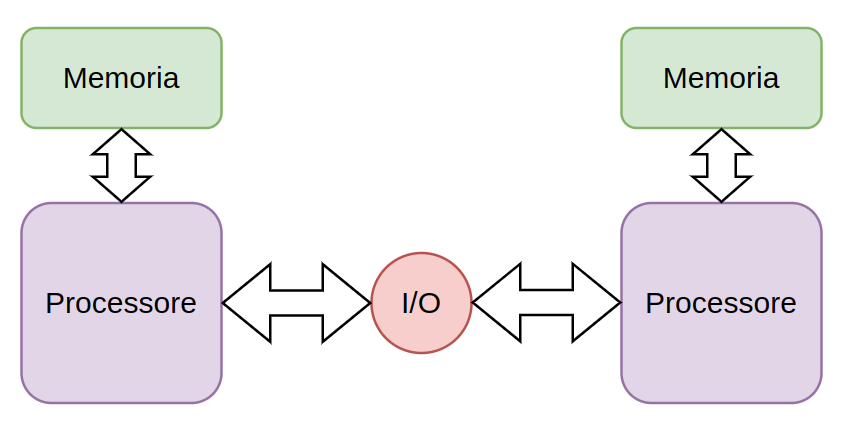
\includegraphics[width=.5\textwidth]{img/P-IO-P.png}
    \caption{Sistemi "gemelli" o sistema multicomputer}\label{img:multi-computer}
\end{figure}

\begin{figure}
    \centering
    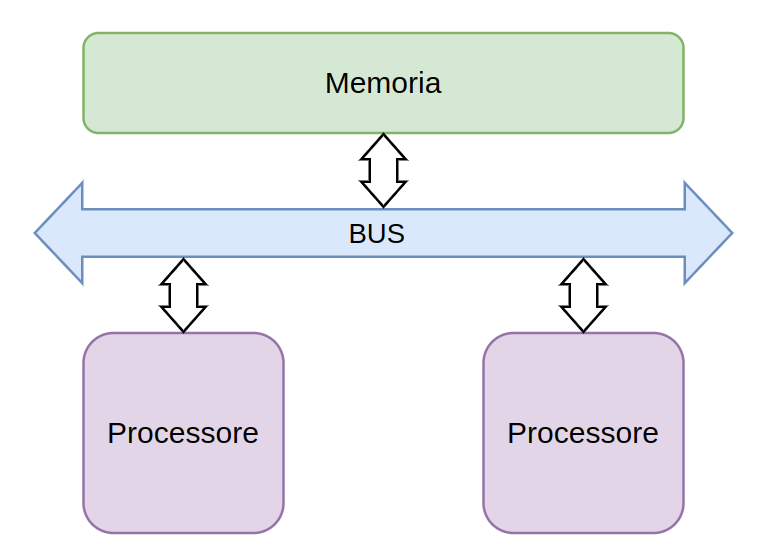
\includegraphics[width=.5\textwidth]{img/P-BUS-P.png}
    \caption{Sistema a memoria condivisa}\label{img:shared-memory}
\end{figure}

\begin{figure}
    \centering
    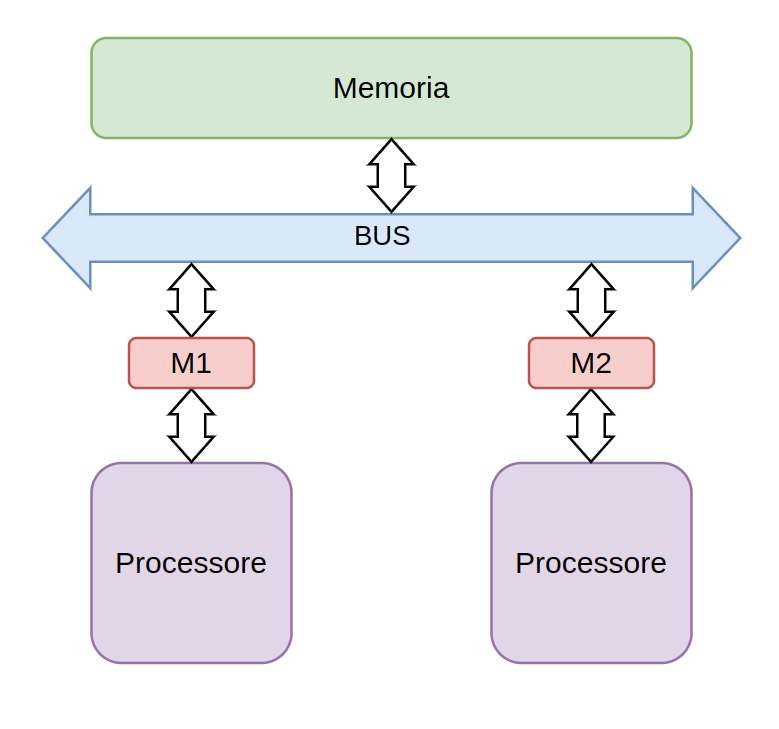
\includegraphics[width=.5\textwidth]{img/P-M-BUS-M-P.png}
    \caption{Sistema multicore}\label{img:multi-core}
\end{figure}

I sistemi che sfruttano le gerarchie di memoria prendono il nome di \textbf{sistemi multicore}, che non hanno solo 2 livelli di gerarchia di memoria, ma ne hanno vari, in base ai casi.

\newpage
\subsection{Multi-Computer e Multi-Processore}
Concentriamo la nostra attenzione sui sistemi MIMD. Escludendo la possibilità di avere un parallelismo interno, è possibile individuare due categorie di sistemi che permettono a più processori di lavorare su dati diversi, questi sono detti Multi-Computer e Multi-Processore.
\\
Un primo metodo utile a far interagire due (o più) sistemi differenti è introdurre un intermediario, ovvero un particolare tipo di sistema di I/O che sia efficace e veloce. In tal caso, quanto più rapidi saranno i processori, tanto più dovrà esserlo il sistema (oltre che la rete che li interconnette). La limitazione principale di tale modello è la sensibilità ai limiti tecnologici dovuti all'interconnessione. Il sistema globale è detto \textbf{Multi-Computer} ed è particolarmente utilizzato per applicazioni che richiedono calcoli dedicati [\ref{fig:multi-computer}].
\begin{figure}[!ht]
    \centering
    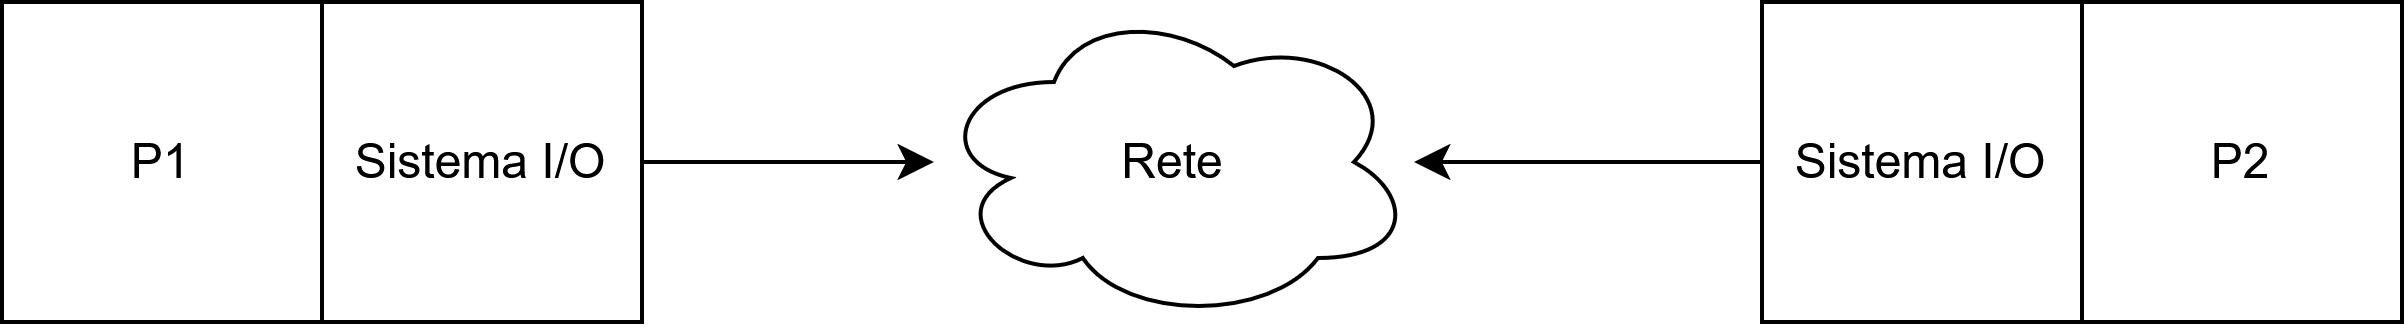
\includegraphics[width=0.8\linewidth]{img/multi-processore.png}
    \caption{Architettura di un sistema Multi-Computer.}
    \label{fig:multi-computer}
\end{figure}

Un'altra possibilità per far interagire i processori è direttamente tramite la memoria, ottenendo un sistema complessivo detto \textbf{Multi-Processore} [\ref{fig:multi-processore}]. In tal caso, la comunicazione tra i processori avviene direttamente tramite bus, superando il problema legato alla fisica realizzabilità di connessioni su larga scala. Il vantaggio di questi sistemi è che i dati possono essere trasferiti molto rapidamente in memoria grazie al bus, mentre lo svantaggio è relativo alla competizione tra i processori negli accessi in memoria. Una possibile miglioria all'architettura proposta consiste nell'integrare a ciascun processore una memoria interna più piccola che gli permetta di gestire le istruzioni. In altre parole, è necessario gestire una gerarchia delle memoria. 
Potremmo (erroneamente) pensare che aggiungere più core permetta di velocizzare il sistema, in realtà questo è sbagliato perché complicherebbe notevolmente le connessioni del bus, il quale diventerebbe il collo di bottiglia del modello.
\begin{figure}[!ht]
    \centering
    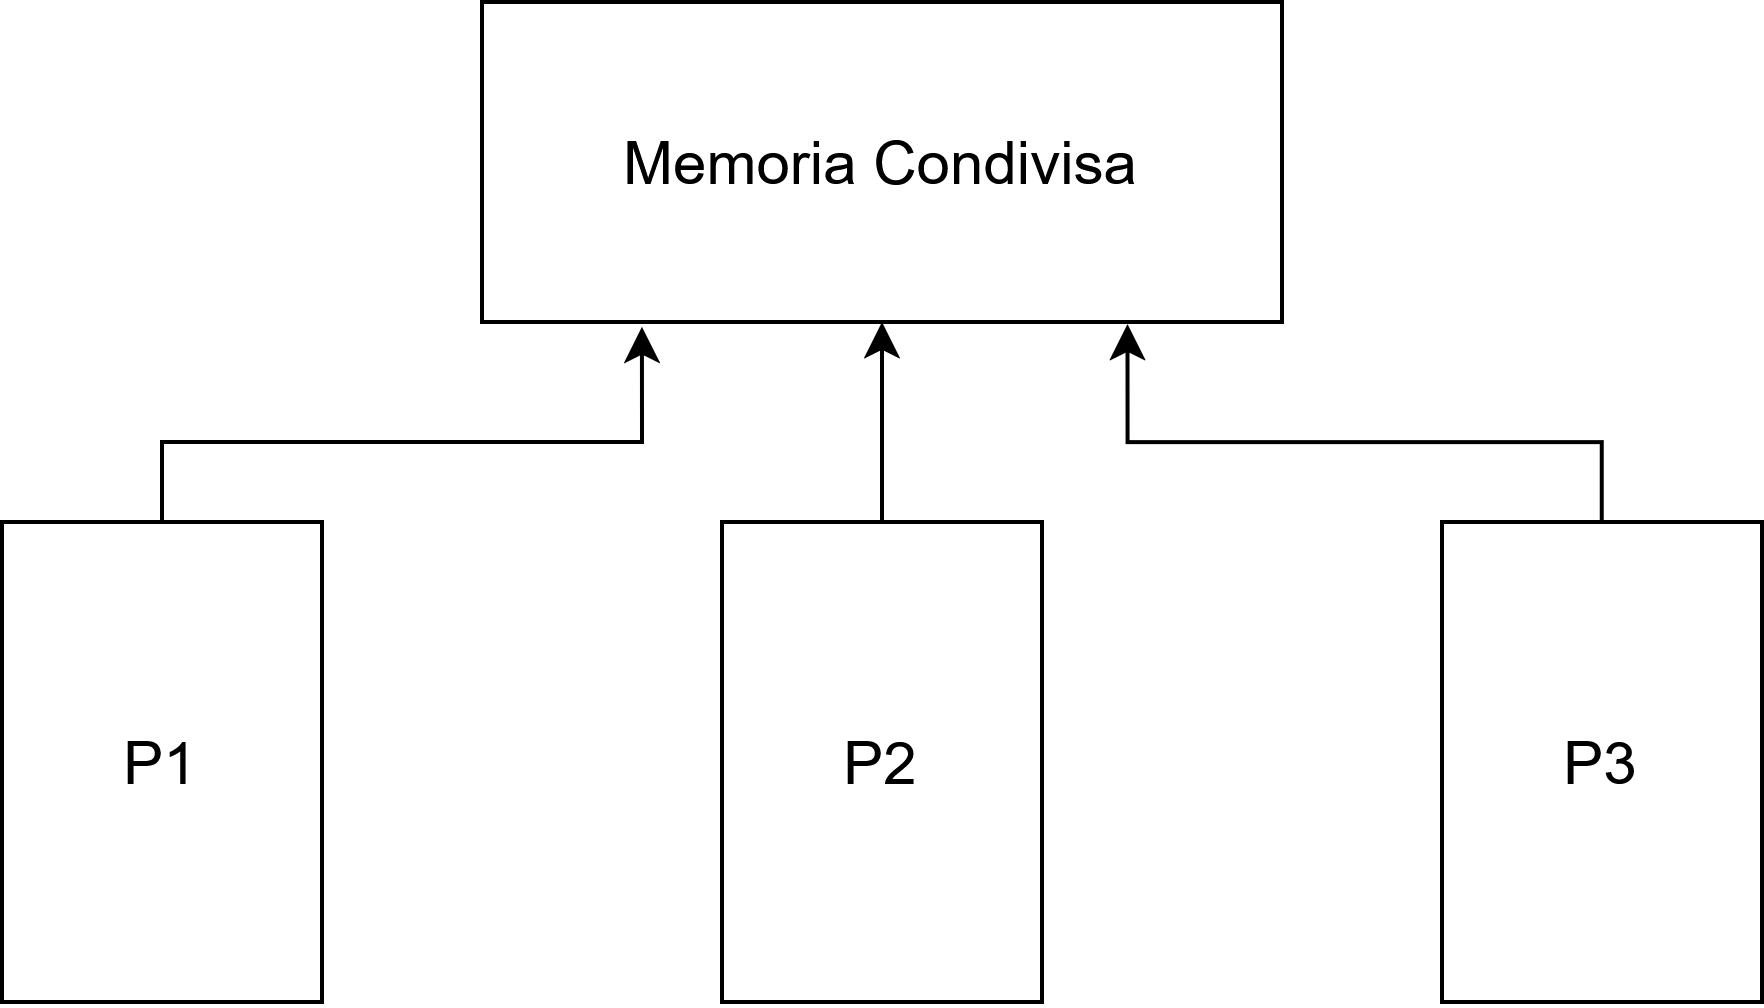
\includegraphics[width=0.5\linewidth]{img/multi-computer.png}
    \caption{Architettura di un sistema Multi-Processore.}
    \label{fig:multi-processore}
\end{figure}
L'esistenza di un modello non esclude la possibilità di inserirne un altro, cosa che accade tipicamente nei sistemi moderni.

\subsection{Speed Up}
La \textbf{legge di Amdhal} afferma che il tempo di calcolo di un programma è dato da: 
\[t_s=t_{ss}+t_{sp}\]
Ovvero, la somma tra il tempo di esecuzione di una parte del programma che è strettamente seriale e il
tempo di esecuzione della parte del programma che è parallelizzabile. In altre parole, la legge dice che una macchina parallela può essere veloce quanto si vuole, ma ci sarà sempre una parte del codice che non è parallelizzabile e che quindi rallenterà l'esecuzione. Un parametro che ci permette di valutare se risulta conveniente ricorrere a un'architettura parallela è lo \textbf{speed-up}, che rappresenta il guadagno che si quantifica con una macchina parallela rispetto all'utilizzo di una macchina puramente sequenziale: 
\[S=\frac{T_{SEQ}}{T_{PAR}} \rightarrow N \space (teorico)\]
Dove \(N\) è il numero di unità di calcolo. Il limite riportato è puramente teorico poiché non tiene conto dell'interazione necessaria fra i nodi, che richiede sicuramente ulteriore tempo. Volendo quindi essere più precisi, dunque, la formula precedente va corretta nel seguente modo:
\[S=\frac{T_{SEQ}}{T_{SEQ}/N+T_{INT}}=\frac{1}{1+\frac{T_{INT}}{T_{SEQ}}N}N \space \space (*)\]
Dove \(T_{INT}\) è il tempo di interazione citato. Dalla seconda espressione, è evidente che per convergere allo speed-up teorico è necessario che il termine \(\frac{T_{INT}}{T_{SEQ}}N<<1\). Possiamo ulteriormente modificare il termine:
\[\frac{T_{INT}}{T_{SEQ}}N=\frac{T_{INT}}{\frac{T_{SEQ}}{N}}=\frac{T_{INT}}{T_{CalcP}}\]
Dove \(T_{CalcP}\) è un termine che ingloba il solo calcolo parallelo senza interferenze. Da questo, è evidente (come potevamo immaginare) che se si calcola poco e si spreca molto tempo nelle interazioni risulta impossibile convergere allo speed-up teorico. L'equazione (*) è fondamentale, in quanto lega il problema (tempo di calcolo parallelo, quanto calcolo bisogna fare) con la tecnologia (tempo di interazione necessario per scambiare i dati, dipendente dalla velocità della rete). Una facile conseguenza di questo è che se abbiamo dei processori molto lenti e bisogna fare molto calcolo, la rete può essere anche poco veloce perché in questa situazione non si trae alcun vantaggio dalla velocità della rete, se invece bisogna fare poco calcolo e i processori sono veloci, allora la rete deve essere veloce. Questo concetto viene in genere chiamato \textit{grain size}.
\\
\\
Altro parametro spesso usato per valutare la convenienza di un'architettura parallela è l'efficienza, definita come il rapporto fra lo speed-up ed N:
\[\epsilon=\frac{S}{N}=\frac{1}{1+\frac{T_{INT}}{T_{CalcP}}}=\frac{1}{1+a}\approx1-a\rightarrow1\]
In tutti i rami dell'ingegneria l'efficienza (o rendimento) rappresenta sempre \textit{"quanto si guadagna rispetto a
quanto di spende"}. Se \(a\) è piccolo l'efficienza è approssimabile secondo Taylor ad \(1-a\) , da questo si
capisce che l'efficienza è legata al rapporto tra il tempo di interazione ed il tempo di calcolo
parallelo. In più, se il tempo di interazione fosse (idealmente) \(0\), si raggiungerebbe il limite teorico
dell'efficienza (\(1\)). Tuttavia, come abbiamo visto questo risulta impossibile secondo Amdhal.
\\
\\
Ricordiamo che per poter eseguire un programma con la programmazione parallela, e quindi risolvere un
problema che di solito ha una soluzione sequenziale in modo parallelo, devono essere valide la \textit{proprietà commutativa} e la \textit{proprietà
associativa}. Queste due proprietà assicurano la possibilità di poter scomporre e calcolare separatamente le soluzioni a sottoproblemi, per poi ricomporle ottenere la soluzione finale.
\\
\\
Per mostrare un'esempio applicativo, consideriamo  le due matrici \(A\) e \(B\) con dimensione \(4x4\), e ipotizziamo di volerne fare il prodotto riga per
riga. Quindi, l'elemento \(C_{ij}\) della matrice risultato \(C\), è il prodotto scalare fra due righe delle matrici: \(C_{ij}=R_{iA} \cdot R_{jB}\). Le due proprietà associativa e commutativa valgono senza dubbio, per cui il prodotto matriciale è sicuramente adatto per il calcolo parallelo. Inoltre, non c'è bisogno di una fase di comunicazione fra i diversi nodi. Potremmo suddividere il
lavoro tra due macchine dando ad ognuna la matrice \(B\) e una coppia di vettori riga di \(A\) (ad esempio \(A1,A2\) e \(A3,A4\)). In questo caso, il costo di interferenza è \(0\) e proprio per questo motivo l'efficienza è \(1\). Se aumentiamo il numero di processori da 2 a 4, affidando ad ogni processore il compito di fare il prodotto tra \(B\) ed un unico vettore di \(A\), l'efficienza resta \(1\), quello che cambia è lo speed-up. Per il caso a due processori è \(2\), mentre diventa \(4\) nel caso a quattro processori. Da
questi due semplici casi si potrebbe pensare di aumentare il numero di processori così da ottenere uno speed-up sempre crescente. La considerazione è certamente vera, però c'è lo svantaggio dell'occupazione della memoria, in quanto ad ogni processore bisogna
affidare una copia della matrice \(B\) ed un vettore di \(A\). In generale bisogna sempre fare i conti con le risorse disponibili nel sistema, mentre la soluzione proposta sembra ignorare del tutto questa regola. 
\\
\\
Una seconda possibile soluzione al problema proposto consiste nel suddividere entrambe le matrice sulle due macchine a disposizione. Nonostante questo permetta di risparmiare in termini di memoria, ci sarà sicuramente un'influenza sull'efficienza. In tal caso, le due macchine devono scambiarsi informazioni sulle righe delle matrici per completare il calcolo, per cui sarà necessario un tempo di interazione. In questa soluzione, il DMA si rende sicuramente utile.
\\
\\
Una terza ed ultima soluzione consiste nell'utilizzo di un'architettura su più nodi (multicomputer), su ciascuno dei quali possiamo risolvere i prodotti \(C_{ii}=A_{ii}\cdot B_{ii}\). Il problema è che in tal modo stiamo popolando la sola diagonale principale della matrice \(C\), per poter ottenere il risultato completo è necessario ruotare in ognuno dei nodi la riga di \(B\).
\begin{figure}[!h]
    \centering
    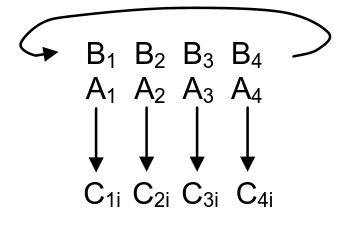
\includegraphics[width=0.3\linewidth]{img/matrix.png}
    \caption{Calcolo parallelo della matrice \(C\) su \(4\) nodi.}
    \label{fig:matrix}
\end{figure}


\subsection{Coerenza della memoria cache nelle architetture parallele}
In generale, l'obbiettivo che si pone nella realizzazione di un'architettura è quello di diminuire i costi di interazione senza agire sul software, ma solo sull'hardware. Ricordiamo che il costo di interazione è il carico introdotto dalla comunicazione per lo scambio di informazioni che avviene tra due o più processi.
\\
\\
Per un sistema multiprocessore, tale costo è determinato dal carico a cui è sottoposto il bus comune con cui i processi interagiscono per accedere alla memoria condivisa. Al fine di diminuire l'iterazione tra i processi, è necessario introdurre, come sarà discusso nel capitolo sulle memorie [\ref{}], una gerarchia di memorie. Ciò si traduce nel
fornire ai diversi processori una propria memoria più veloce di quella comune, quindi una \textit{memoria cache} [\ref{fig:mulproc-mem}].
\begin{figure}[!h]
    \centering
    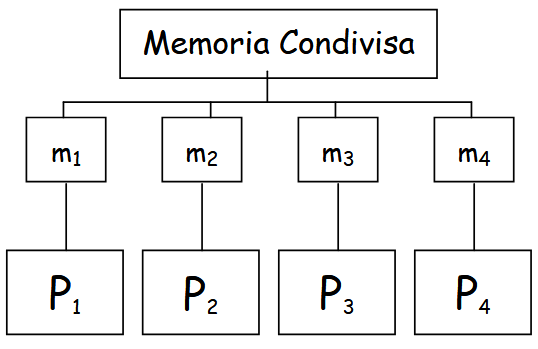
\includegraphics[width=0.3\linewidth]{img/multiproc-gerarchia.png}
    \caption{Sistema multiprocessore con gerarchia delle memorie.}
    \label{fig:mulproc-mem}
\end{figure}
Con la soluzione illustrata, però, nasce un problema di gestione della \textbf{coerenza della memoria} condivisa. Non tanto per le istruzioni eseguite dai diversi processori, le quali devono essere solamente lette, ma per i dati condivisi che possono essere modificati.
Il problema può essere affrontato tramite due strategie:
\begin{itemize}
    \item \textbf{Write Through}: Ogni qual volta un dato viene modificato, il suo valore viene immediatamente aggiornato in memoria condivisa.
    \item \textbf{Write Back}: Le modifiche non sono riportate immediatamente, ma in un secondo momento.
\end{itemize}
Per entrambe le tecniche, si necessita quindi di una politica di \textit{invalidazione dei dati modificati} da
un processo, i quali possono essere presenti nelle cache di altri processori o della memoria
comune. Ovviamente, nel caso della write through, la memoria condivisa viene aggiornata immediatamente, per cui non possiede mai valori da invalidare. Tutto ciò porta a un'ulteriore sovraccarico del bus comune.
\\
\\
Concentriamoci prima sulla soluzione adottata da write through. Per capirne il funzionamento, supponiamo che ci siano i due processori \(P_i\) (spia) e \(P_j\) (spiato) che operano sugli stessi dati. In particolare, osserviamo il processo dal punto di vista del processore spia a fronte delle azioni compiute sui dati sia da se stesso che dall'altro processore. Ogni dato presente in cache, può assumere solo due stati: \textit{valido} e \textit{non valido} [\ref{fig:automa-wt}].
\begin{figure}[!h]
    \centering
    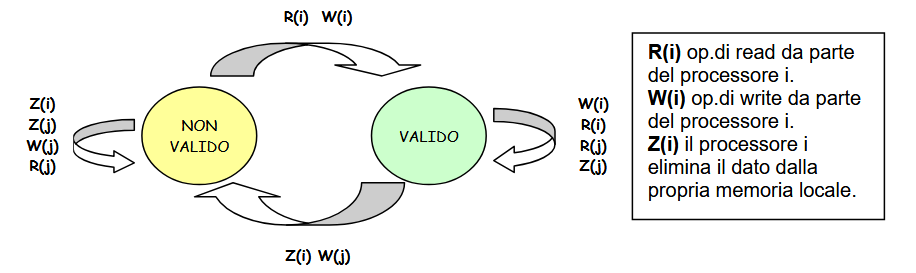
\includegraphics[width=0.55\linewidth]{img/automa_wt.png}
    \caption{Automa per la gestione della coerenza in write through.}
    \label{fig:automa-wt}
\end{figure}
Passiamo ora a considerare il caso write back, in cui bisogna tenere conto che l'aggiornamento del dato in
memoria comune non avviene subito ma in un secondo momento.  
\begin{figure}[!h]
    \centering
    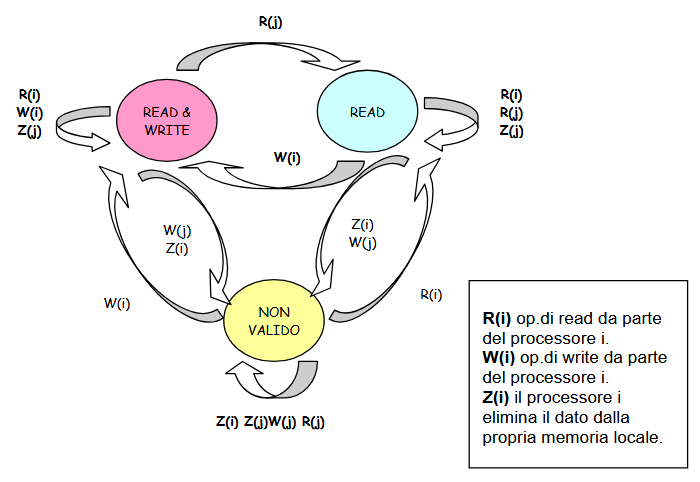
\includegraphics[width=0.55\linewidth]{img/automa-wb.png}
    \caption{Automa per la gestione della coerenza in write back.}
    \label{fig:automa-wb}
\end{figure}

Lo stato \textit{RW} è quello in cui \(P_i\)
può effettuare qualunque tipo di operazione sul dato. Se \(P_j\) legge il dato, si va in uno stato \textit{RO}
(read only), in cui si deve tener conto del fatto che adesso anche altri processori stanno leggendo il dato in
questione e affinché questo sia possibile bisogna effettuare un flush in memoria comune. Da questo stato non si esce mai fintantoché i vari processori si limitano a leggere il dato.
Una eventuale riscrittura da parte di \(P_i\) riporta allo stato \textit{RW}. Questa operazione corrisponde a
invalidare il dato dal punto di vista di \(P_j\). Possiamo rendercene conto osservando il grafo: sia dallo stato \textit{RW} che dallo stato \textit{RO}, l'operazione \(W(j)\) porta sempre nello stato
\textit{NV} dal punto di vista di \(P_i\). Da qui si capisce che entrambi gli stati (\textit{RO} e \textit{RW})
rappresentano la validità del dato in memoria. Quindi, in regime write back una qualunque operazione
di scrittura dal parte di un processore rende il dato invalido per tutti gli altri, come d'altra parte è ovvio. Da uno stato invalido si può tornare se \(P_i\) legge o scrive il dato. In particolare, \(R(i)\) porta in \textit{RO}, e \(W(i)\) in \textit{RW}. Ci si potrebbe domandare perché sono stati distinti i due stati, entrambi validi, \textit{RW} e \textit{RO}. Il motivo è che nel caso in cui da \textit{NV} si passa a \textit{RW}, il processore \(P_i\) si limita ad
aggiornare nella propria memoria locale. Se invece si passa ad \textit{RO}, si forza il sistema di
gestione a prelevare il dato dalla memoria centrale e a scaricarlo nella cache di \(P_i\). Le due situazioni sono quindi sostanzialmente diverse. Da quanto detto, lo stato che risulta più critico per il sistema è quello di \textit{RW}, dove i dati modificati dal processore \(P_i\) sono validi solo per se stesso, e quindi non allineati alla memoria condivisa.
\\
\\
Oltre alle tecniche standard di write through e write back, è stata ideata un’ulteriore tecnica detta di \textit{write once}, nella quale la prima volta viene eseguito il write through e se in seguito è necessario effettuare altre scritture sullo stesso dato, si passa alla modalità write back, in modo da
evitare di appesantire il traffico sul bus. Osserviamo che l’automa a stati finiti per la write once richiede 4 stati [\ref{fig:automa-wo}].
\begin{figure}[!h]
    \centering
    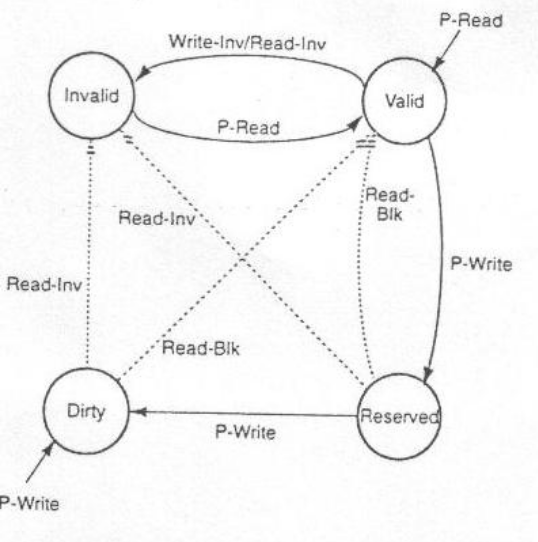
\includegraphics[width=0.5\linewidth]{img/automa-wo.png}
    \caption{Automa per la gestione della coerenza in write once.}
    \label{fig:automa-wo}
\end{figure}
Un'ultima tecnica per la coerenza fa uso di \textit{puntatori}. \MakeUppercase{è} presente una shared memory che indica in ogni istante in quale cache è presente un certo dato, e i puntatori consentono di accedervi. Quando una cache invalida il dato, invece di spostare fisicamente i dati, si possono usare i puntatori per creare delle catene logiche che consentono di andare a prendere sempre la versione corretta del dato. Osserviamo che la macchina non sa e non deve preoccuparsi di dove si trovano i dati validi, tutto è gestito dall'hardware.
